% Tags: 4321102, table, asynchronous, counter, logic, 4-bit
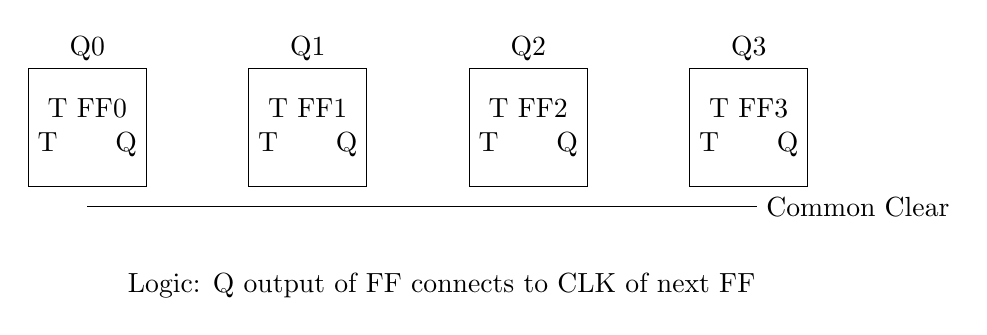
\begin{tikzpicture}[
    node distance=2.5cm,
    auto,
    block/.style={rectangle, draw, minimum width=1.5cm, minimum height=1.5cm, align=center}
]
    \foreach \i in {0,1,2,3} {
        \node[block] (TFF\i) at (\i*2.8, 0) {T FF\i\\T \hspace{0.5cm} Q};
        \node at (\i*2.8, 1) {Q\i};
    }
    
    \node at (4.5, -2) {Logic: Q output of FF connects to CLK of next FF};
    \draw (0, -1) -- (8.5, -1) node[right] {Common Clear};

\end{tikzpicture}
